\documentclass[journal]{IEEEtran}

\usepackage{amsmath,amssymb,amsfonts}
\usepackage{mathptmx}
\usepackage{booktabs}
\usepackage{array}
\usepackage{graphicx}
\usepackage{textcomp}
\usepackage{url}
\usepackage{tikz}
\usetikzlibrary{shapes,arrows.meta,positioning,fit,calc}
\usepackage[hidelinks]{hyperref}

\begin{document}

\title{A Memory-Efficient FPGA Implementation and Hardware/Software Co-Design of Post-Quantum HQC-128 for Resource-Constrained Edge Devices}

\author{Arnav~Pillai%
\thanks{The author is with the Department of Electrical and Electronics Engineering, BITS Pilani, K.~K.~Birla Goa Campus, Goa 403726, India (e-mail: f20240673@goa.bits-pilani.ac.in).}}

\maketitle

\begin{abstract}
Deploying the National Institute of Standards and Technology (NIST) Hamming Quasi-Cyclic (HQC-128) cryptosystem on edge nodes requires hardware accelerators that fit within tight on-chip memory limits. Most prior full-KEM and decapsulation field-programmable gate array (FPGA) designs consume 17.5 to 62.5 Block RAM (BRAM) tiles, which occupies up to 125\% of the 50-BRAM capacity on an AMD Artix-7 xc7a35t. This letter presents a memory-efficient hardware/software co-design for HQC-128 public-key encryption (PKE). An interval conflict graph of polynomial lifetimes ($\chi(G) = 6$) fits all 14 variables into 6.0 RAMB36 tiles and 408 distributed lookup table (LUT) RAMs. Three 64-bit ring multipliers time-share a dual-port accumulator alongside a Chien-search and Forney Reed-Solomon codec. On an Artix-7 xc7a35t-1, the routed core occupies 8,246 LUTs, 7,868 flip-flops, 6.0 BRAMs (12.0\%), and 0 digital signal processing (DSP) slices. At 119.0~MHz, the core consumes 0.158~W and 118.5~$\mu$J per KeyGen+Encrypt+Decrypt sequence (0.750~ms, 89,262 cycles). Compute cycles drop by $2,949\times$ for PKE ($1,951\times$ for Fujisaki--Okamoto key encapsulation [FO-KEM]) relative to 32-bit RISC-V software.
\end{abstract}

\begin{IEEEkeywords}
Edge devices, field-programmable gate array (FPGA), Hamming Quasi-Cyclic (HQC), hardware/software co-design, post-quantum cryptography (PQC).
\end{IEEEkeywords}

\section{Introduction}
\IEEEPARstart{L}{arge-scale} quantum computers running Shor's algorithm solve integer factorization and discrete logarithms in polynomial time and break RSA and elliptic-curve schemes. Alongside the lattice-based ML-KEM standard (NIST FIPS~203), the National Institute of Standards and Technology (NIST) selected Hamming Quasi-Cyclic (HQC)~\cite{melchor2023hqc, nist2025ir8545} in March 2025 for standardization as a code-based alternative based on syndrome decoding over quasi-cyclic codes. Unlike Classic McEliece (public keys $>260$~KB), HQC-128 uses a 2,249-byte public key and bounds the decryption failure rate (DFR) below $2^{-128}$ for bandwidth-limited edge telemetry. However, HQC-128 operates on binary polynomials of degree $N = 17,669$ in cyclic ring $\mathcal{R} = \mathbb{F}_2[X]/(X^N - 1)$ and decodes concatenated shortened Reed-Solomon (RS) and duplicated Reed-Muller (RM) codes.

On a 32-bit embedded RISC-V processor (CV32E40P), pure software execution of HQC-128 takes 263.3~million cycles (43.6M key generation, 87.6M encapsulation, 132.1M decapsulation)~\cite{ras2025optimizing}, where 17,669-bit polynomial multiplication accounts for ${\approx}95\%$ of runtime. Offloading HQC to an entry-level FPGA System-on-Chip (SoC) such as the AMD Artix-7 xc7a35t (UG473, 20,800 LUTs, 50 BRAM tiles) removes this bottleneck only if the accelerator leaves the vast majority of on-chip BRAM available for host RISC-V memories and queues. Most HQC-128 FPGA cores exceed this budget: Deshpande et al.~\cite{deshpande2023fast} use 20.0--24.0 BRAMs; Antognazza et al.~\cite{antognazza2024high} use 20.0--20.5 BRAMs per primitive; Tu and Xie (LEAH)~\cite{tu2024leah} use 7.0, 12.5, and 17.5 BRAMs across cores; and Wang et al.~\cite{wang2024high} use 62.5 BRAMs (125\% of an xc7a35t). Earlier co-designs such as Sch{\"o}ffel et al.~\cite{schoeffel2022code} use 3.0 BRAMs and 0 DSPs, but take 1.30~ms for encapsulation and 5.60~ms for decapsulation.

Because edge SoCs include a host CPU for networking, dedicated fabric Keccak sponges are unnecessary. We partition HQC-128 into a HW/SW co-design: the host CPU runs SHAKE256 (FIPS~202) seed expansion and index sampling in software, while a unified FPGA coprocessor executes all three PKE primitives (\textit{KeyGen}, \textit{Encrypt}, \textit{Decrypt}) in 6.0 RAMB36 tiles. Our contributions are:
\begin{enumerate}\setlength{\itemsep}{0pt}\setlength{\parsep}{0pt}\setlength{\parskip}{0pt}
    \item \textit{Memory-Lifetime Conflict Bound:} We model all 14 logical buffers (7 dense polynomials, 3 accumulators, and 4 sparse arrays) as an interval conflict graph $G$ with $\chi(G) = \omega(G) = 6$. In-place aliasing ($\mathbf{u} \leftrightarrow \mathbf{n}$, $\mathbf{v} \leftrightarrow \mathbf{mG}$), a shared accumulator ($\mathbf{T}_1$), and distributed LUTRAM (408 LUTs) reduce storage to 6.0 RAMB36 and 0 RAMB18 tiles.
    \item \textit{64-Bit vs. 72-Bit Word-Width Analysis and Codec:} We show analytically why a 64-bit datapath avoids the addressing and alignment penalties of native 72-bit RAMB36 ports for $N=17,669$ ring folding and $17,664$-bit RS-RM codewords, and integrate 64-bit circular shifters with a Chien-search and pipelined Forney RS decoder verified across 100 NIST vectors.
    \item \textit{SAIF-Annotated Power and Energy Scaling:} Post-route power analysis with 100-vector simulation switching activity on Artix-7 xc7a200t-2 and xc7a35t-1 shows that running the xc7a35t-1 core at $119.0$~MHz amortizes static power and cuts total PKE energy by 66.5\% (to 118.5~$\mu$J) relative to 25~MHz.
    \item \textit{AXI4-Lite SoC Co-Design:} An AXI4-Lite bridge (153 LUTs, 293 FFs) and C99 driver interface the core to complete PKE computation in 0.750~ms (89,262 core cycles, or 134,939 with FO re-encryption), leaving 88.0\% of xc7a35t BRAMs free.
\end{enumerate}

\section{HQC-128 Preliminaries and Bottlenecks}

\subsection{HQC-128 Public-Key Encryption}
Let $\mathbb{F}_2$ denote the binary field and $\mathcal{R} = \mathbb{F}_2[X]/(X^N - 1)$ the cyclic ring with prime $N = 17,669$. Bold lowercase letters denote $N$-bit polynomials in $\mathcal{R}$, and $\mathcal{R}_\omega \subset \mathcal{R}$ denotes sparse polynomials of Hamming weight $\omega$. In HQC-128~\cite{melchor2023hqc}, secret polynomials use $\omega = 66$ and ephemeral encryption polynomials use $\omega_r = \omega_e = 75$ ($\text{DFR} < 2^{-128}$).

\textit{PKE.KeyGen:} From public $\mathbf{h} \in \mathcal{R}$ and secret sparse $\mathbf{x}, \mathbf{y} \in \mathcal{R}_{66}$, key generation computes $\mathbf{s} = \mathbf{x} + \mathbf{h} \cdot \mathbf{y} \in \mathcal{R}$.

\textit{PKE.Encrypt:} A 128-bit message $\mathbf{m} \in \mathbb{F}_2^{128}$ is encoded by an outer shortened $\mathrm{RS}[n_1=46, k_1=16, d_1=31]$ code over $\mathbb{F}_{2^8}$ and an inner duplicated $\mathrm{RM}[n_2=384, k_2=8, d_2=192]$ code (multiplicity 3) to form $\mathbf{mG} \in \mathbb{F}_2^{17,664}$. With ephemeral $\mathbf{r}_1, \mathbf{r}_2, \mathbf{e} \in \mathcal{R}_{75}$, ciphertext $(\mathbf{u}, \mathbf{v})$ is evaluated in $\mathcal{R}$ as $\mathbf{u} = \mathbf{r}_1 + \mathbf{h} \cdot \mathbf{r}_2$ and $\mathbf{v} = \mathbf{mG} + \mathbf{s} \cdot \mathbf{r}_2 + \mathbf{e}$.

\textit{PKE.Decrypt:} Using secret key $\mathbf{y} \in \mathcal{R}_{66}$, decryption computes $\mathbf{n} = \mathbf{v} - \mathbf{u} \cdot \mathbf{y} = \mathbf{mG} + (\mathbf{x} \cdot \mathbf{r}_2 - \mathbf{y} \cdot \mathbf{r}_1 + \mathbf{e}) \in \mathcal{R}$, and decodes its first $17,664$ bits via a Fast Walsh-Hadamard Transform (FWHT) RM decoder and Berlekamp-Massey/Forney RS decoder to recover $\mathbf{m}' \in \mathbb{F}_2^{128}$. In full HQC-128 key encapsulation (KEM), FO decapsulation follows \textit{PKE.Decrypt} with re-encryption (\textit{PKE.Encrypt}).

\subsection{Causes of High BRAM Usage in Existing Hardware}
Although one polynomial in $\mathcal{R}$ holds 17,669~bits ($2,209$~bytes, $<50\%$ of a 36-Kb RAMB36E1), prior HQC-128 cores consume 17.5--62.5 BRAMs due to three factors: 1)~\textit{Wide-Port Fragmentation:} Designs using 128-bit TDP memories~\cite{deshpande2023fast, antognazza2024high} stripe each polynomial across four RAMB36E1 tiles ($4 \times 36 \ge 128$), consuming 20.0 BRAMs for five buffers while leaving $>75\%$ of bit cells unused. 2)~\textit{Private Accumulators and Buffers:} Unified designs~\cite{deshpande2023fast, wang2024high} allocate separate scratchpad BRAMs per primitive and maintain distinct memories for $\mathbf{mG}, \mathbf{v}, \mathbf{u}$, and $\mathbf{n}$. 3)~\textit{Shallow Tables in BRAM:} Sparse vectors ($\le 75 \times 15$-bit $= 1,125$~bits) and $\mathbb{F}_{2^8}$ lookup tables (128--256~bytes) mapped to Block RAM~\cite{deshpande2023fast, wang2024high} waste over a dozen BRAMs on sub-kilobyte arrays.

\section{Proposed HW/SW Co-Design Architecture}

\begin{table}[t]
\centering
\caption{Post-Route Implementation and SAIF Power Metrics across Artix-7 Targets}
\label{tab:target_comp}
\resizebox{\columnwidth}{!}{%
\begin{tabular}{lrr}
\toprule
\textbf{Metric} & \textbf{Artix-7 xc7a200t-2} & \textbf{Artix-7 xc7a35t-1} \\
\midrule
Slice LUTs (Logic / Memory) & 8,246 (7,838 / 408) & 8,246 (7,838 / 408) \\
Slice Registers (FF) & 7,868 (2.9\%) & 7,868 (18.9\%) \\
Block RAM (RAMB36E1) & \textbf{6.0} (1.6\%) & \textbf{6.0} (\textbf{12.0\%}) \\
DSP48E1 Slices & \textbf{0} (0.0\%) & \textbf{0} (0.0\%) \\
Routed WNS (@100.0~MHz) & $+2.410$~ns ($T_{\text{crit}}=7.590$~ns) & $+1.641$~ns ($T_{\text{crit}}=8.359$~ns) \\
Post-Route Extrapolated $F_{\max}$ (Sweep)* & 131.8~MHz (eval. @ 131.0~MHz) & 119.6~MHz (eval. @ 119.0~MHz) \\
\midrule
Power @100~MHz (Dyn/Stat) & 0.202~W (0.080/0.122~W) & 0.146~W (0.078/0.069~W) \\
Power @Swept $F_{\max}$ (Dyn/Stat) & 0.222~W (0.100/0.122~W) & 0.158~W (0.089/0.069~W) \\
PKE Energy (@100~MHz) & 180.3~$\mu$J (0.893~ms) & 130.3~$\mu$J (0.893~ms) \\
PKE Energy (@Swept $F_{\max}$) & 151.3~$\mu$J (0.681~ms) & \textbf{118.5~$\mu$J} (0.750~ms) \\
\bottomrule
\end{tabular}%
}
\vspace{2pt}
{\scriptsize *Extrapolated from routed critical path $T_{\text{crit}} = 10.0\,\text{ns} - \text{WNS}$; power and latency are evaluated at 131.0 and 119.0~MHz.\par}
\end{table}

\begin{table*}[t]
\centering
\caption{Comparison with Prior Hardware Implementations of HQC-128 on Artix-7 FPGAs}
\label{tab:prior_art}
\resizebox{\textwidth}{!}{%
\begin{tabular}{lllrrrrrrr}
\toprule
\textbf{Design} & \textbf{Platform} & \textbf{Scope} & \textbf{LUTs} & \textbf{FFs} & \textbf{BRAM} & \textbf{DSP} & \textbf{$F_{\max}$} & \textbf{Latency (ms)} & \textbf{Energy} \\
 & \textbf{(Device / Speed)} & \textbf{(SHAKE256)} & & & \textbf{(36k)} & & \textbf{(MHz)} & \textbf{KG / Enc / Dec (FO-Dec)} & \\
\midrule
Sch{\"o}ffel et al.~\cite{schoeffel2022code} (Co-Design) & xc7a100t [NR] & KEM Co-Des. (SW) & ${\sim}8,000$ & 2,400 & 3.0 & 0 & 100 & 0.56 / 1.30 / (5.60) & NR \\
Deshpande et al.~\cite{deshpande2023fast} (Balanced) & xc7a100t-3 & Full KEM (HW) & 13,865 & 6,897 & 22.0 & 8 & 164 & 0.10 / 0.20 / (0.29) & NR \\
Deshpande et al.~\cite{deshpande2023fast} (HighSpeed) & xc7a100t-3 & Full KEM (HW) & 15,214 & 7,293 & 24.0 & 8 & 178 & 0.09 / 0.13 / (0.21) & NR \\
Deshpande et al.~\cite{deshpande2023fast} (Decap Only) & xc7a200t-3 & Decap Only (Excluded) & 8,984 & 6,596 & 20.0 & 4 & 192 & -- / -- / (0.251) & NR \\
Antognazza et al.~\cite{antognazza2024high} (KeyGen) & xc7a200t-3* & KeyGen Only (Excluded) & 6,827 & 5,444 & 20.0 & 0 & 208 & 0.030 / -- / -- & NR \\
Antognazza et al.~\cite{antognazza2024high} (Encap) & xc7a200t-3* & Encap Only (Excluded) & 7,064 & 6,378 & 20.0 & 0 & 168 & -- / 0.079 / -- & NR \\
Antognazza et al.~\cite{antognazza2024high} (Decap) & xc7a200t-3* & Decap Only (Excluded) & 13,327 & 9,488 & 20.5 & 0 & 167 & -- / -- / (0.119) & NR \\
Tu \& Xie (LEAH)~\cite{tu2024leah} (KeyGen) & xc7a200t [NR] & KeyGen Only (HW) & 2,834 & 1,626 & 7.0 & 0 & 218 & 0.052 / -- / -- & NR \\
Tu \& Xie (LEAH)~\cite{tu2024leah} (Encap) & xc7a200t [NR] & Encap Only (HW) & 5,455 & 3,280 & 12.5 & 0 & 199 & -- / 0.071 / -- & NR \\
Tu \& Xie (LEAH)~\cite{tu2024leah} (Decap) & xc7a200t [NR] & Decap Only (HW) & 9,878 & 10,212 & 17.5 & 0 & 191 & -- / -- / (0.129) & NR \\
Wang et al.~\cite{wang2024high} & xc7a200t-3 & Full KEM (HW) & 20,201 & 13,685 & 62.5 & NR & 157 & 0.079 / 0.114 / (0.207) & NR \\
\midrule
\textbf{This Work (xc7a200t-2 @131~MHz)} & \textbf{xc7a200t-2} & \textbf{Unified PKE (SW)} & \textbf{8,246} & \textbf{7,868} & \textbf{6.0} & \textbf{0} & \textbf{131.8} & \textbf{0.151 / 0.349 / 0.182 (0.530)} & \textbf{151.3~$\mu$J} \\
\textbf{This Work (xc7a35t-1 @119~MHz)} & \textbf{xc7a35t-1} & \textbf{Unified PKE (SW)} & \textbf{8,246} & \textbf{7,868} & \textbf{6.0} & \textbf{0} & \textbf{119.6} & \textbf{0.166 / 0.384 / 0.200 (0.584)} & \textbf{118.5~$\mu$J} \\
\bottomrule
\multicolumn{10}{l}{\footnotesize NR = Not Reported. HW/SW indicates on-chip vs. host-CPU SHAKE256; Excluded indicates benchmark without SHAKE256. Dec (FO-Dec) lists PKE.Decrypt and FO-KEM Decaps ($\text{Dec}+\text{Re-Enc}$). *Validated on xc7a100t-1.}
\end{tabular}%
}
\end{table*}

\begin{figure}[t]
\centering
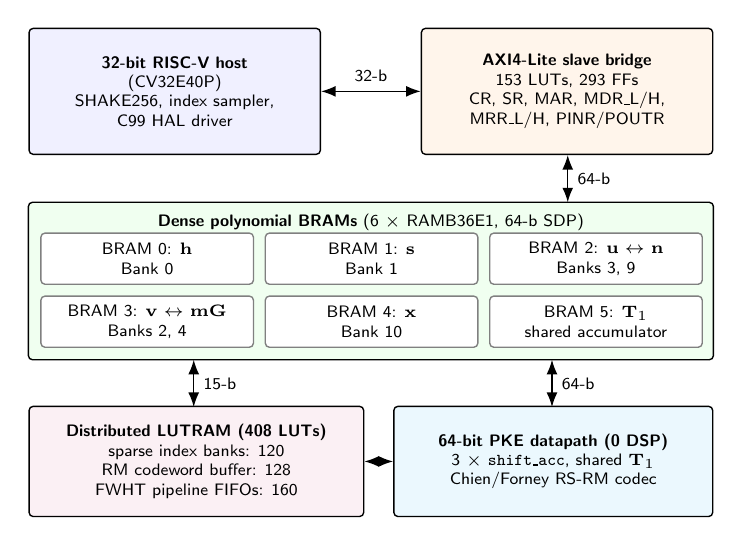
\begin{tikzpicture}[font=\sffamily\fontsize{6}{7}\selectfont, >=Latex,
    box/.style={draw, rounded corners=1.5pt, line width=0.5pt, align=center, inner sep=2pt},
    bus/.style={<->, line width=0.5pt}]
% Row A: host and bridge
\node[box, fill=blue!6, minimum width=3.7cm, minimum height=1.6cm, anchor=south west] (host) at (0,4.6)
  {\textbf{32-bit RISC-V host}\\(CV32E40P)\\SHAKE256, index sampler,\\C99 HAL driver};
\node[box, fill=orange!8, minimum width=3.7cm, minimum height=1.6cm, anchor=south east] (axi) at (8.7,4.6)
  {\textbf{AXI4-Lite slave bridge}\\153 LUTs, 293 FFs\\CR, SR, MAR, MDR\_L/H,\\MRR\_L/H, PINR/POUTR};
\draw[bus] (host.east) -- node[above] {32-b} (axi.west);
% Row B: dense BRAMs
\draw[rounded corners=1.5pt, fill=green!6, line width=0.5pt] (0,2.0) rectangle (8.7,4.0);
\node[anchor=north] at (4.35,3.97) {\textbf{Dense polynomial BRAMs} (6 $\times$ RAMB36E1, 64-b SDP)};
\foreach \x/\a/\b in {0.15/{BRAM 0: $\mathbf{h}$}/{Bank 0}, 3.00/{BRAM 1: $\mathbf{s}$}/{Bank 1}, 5.85/{BRAM 2: $\mathbf{u}\leftrightarrow\mathbf{n}$}/{Banks 3, 9}}
  \node[box, fill=white, draw=gray, minimum width=2.7cm, minimum height=0.65cm, anchor=south west] at (\x,2.95) {\a\\\b};
\foreach \x/\a/\b in {0.15/{BRAM 3: $\mathbf{v}\leftrightarrow\mathbf{mG}$}/{Banks 2, 4}, 3.00/{BRAM 4: $\mathbf{x}$}/{Bank 10}, 5.85/{BRAM 5: $\mathbf{T}_1$}/{shared accumulator}}
  \node[box, fill=white, draw=gray, minimum width=2.7cm, minimum height=0.65cm, anchor=south west] at (\x,2.15) {\a\\\b};
\draw[bus] (6.85,4.6) -- node[right] {64-b} (6.85,4.0);
% Row C: LUTRAM and datapath
\node[box, fill=purple!6, minimum width=4.25cm, minimum height=1.4cm, anchor=south west] (lut) at (0,0)
  {\textbf{Distributed LUTRAM (408 LUTs)}\\sparse index banks: 120\\RM codeword buffer: 128\\FWHT pipeline FIFOs: 160};
\node[box, fill=cyan!8, minimum width=4.05cm, minimum height=1.4cm, anchor=south east] (dp) at (8.7,0)
  {\textbf{64-bit PKE datapath (0 DSP)}\\3 $\times$ \texttt{shift\_acc}, shared $\mathbf{T}_1$\\Chien/Forney RS-RM codec};
\draw[bus] (2.1,2.0) -- node[right] {15-b} (2.1,1.4);
\draw[bus] (6.65,2.0) -- node[right] {64-b} (6.65,1.4);
\draw[bus] (lut.east) -- (dp.west);
\end{tikzpicture}
\caption{HQC-128 HW/SW co-design architecture: 32-bit AXI4-Lite bridge, six lifetime-aliased RAMB36E1 polynomial memories, 408-LUT distributed LUTRAM, and the 64-bit PKE datapath.}
\label{fig:mem_alloc}
\end{figure}

\subsection{Memory-Lifetime Conflict Graph and 6-BRAM Allocation}
Across the five PKE phases ($\Phi_{\text{kg}} \rightarrow \Phi_{\text{enc-codec}} \rightarrow \Phi_{\text{enc-arith}} \rightarrow \Phi_{\text{dec-arith}} \rightarrow \Phi_{\text{dec-codec}}$), the core manages 14 buffers: 7 dense polynomials ($\mathbf{h}, \mathbf{s}, \mathbf{x}, \mathbf{u}, \mathbf{v}, \mathbf{mG}, \mathbf{n}$), 3 accumulators ($\mathbf{T}_{\text{kg}}, \mathbf{T}_{\text{enc}}, \mathbf{T}_{\text{dec}}$), and 4 sparse arrays ($\mathbf{y}, \mathbf{r}_1, \mathbf{r}_2, \mathbf{e}$), as shown in Fig.~\ref{fig:mem_alloc}.

First, four sparse arrays $\mathbf{y}$ ($66 \times 15$-bit) and $\mathbf{r}_1, \mathbf{r}_2, \mathbf{e}$ ($75 \times 15$-bit each) map to distributed LUTRAM, using 120 LUTRAMs (30 per bank). Combined with 128 LUTRAMs for the RM encoder and 160 LUTRAMs for the 7-layer Fast Walsh-Hadamard Transform (FWHT) decoder FIFOs, total distributed memory is 408 LUTRAMs and 0 BRAMs. Dense secret $\mathbf{x}$ resides in BRAM~4; after 64-bit multiplication $\mathbf{h} \cdot \mathbf{y}$ accumulates into $\mathbf{T}_1$ ($66 \times 282 = 18,612$ cycles), \textit{KeyGen} finishes $\mathbf{s} = \mathbf{x} \oplus \mathbf{T}_1$ in 831 cycles ($6.98\ \mu\text{s}$ at 119~MHz, 19,796 total cycles) via a 98-LUT word-wise XOR unit.

Second, we model buffer residency across PKE phases as an interval conflict graph $G = (V, E)$. Disjoint arithmetic phases collapse the three ring accumulators into a shared dual-port BRAM $\mathbf{T}_1$, which forms the 8-vertex dense buffer set $V = \{\mathbf{h}, \mathbf{s}, \mathbf{x}, \mathbf{u}, \mathbf{v}, \mathbf{mG}, \mathbf{n}, \mathbf{T}_1\}$ ($277 \times 64$-bit each). An edge $(u, w) \in E$ exists iff lifetimes overlap: $I(u) \cap I(w) \ne \emptyset$.

\textbf{Theorem 1 (Chromatic Memory Lower Bound):} \textit{Under persistent on-chip keys $\{\mathbf{h}, \mathbf{s}, \mathbf{x}\}$ with SDP Block RAMs, the chromatic number of conflict graph $G$ satisfies $\chi(G) = 6$. Exactly 6.0 RAMB36E1 tiles is minimal and sufficient for stall-free execution.}

\textit{Proof:} An interval graph is chordal and therefore perfect. By the Hajnal-Sur\'anyi theorem on graph coloring, the chromatic number equals the clique number: $\chi(G) = \omega(G)$. During $\Phi_{\text{enc-arith}}$, keys $\{\mathbf{h}, \mathbf{s}, \mathbf{x}\}$ are resident, ciphertext $\mathbf{u} = \mathbf{r}_1 + \mathbf{h} \cdot \mathbf{r}_2$ is held, and $\mathbf{T}_1$ computes $\mathbf{s} \cdot \mathbf{r}_2$. At step $t^*$, codeword $\mathbf{mG}$ is read to form $\mathbf{T}_1 \leftarrow \mathbf{T}_1 \oplus \mathbf{mG}$. Here, all six buffers are simultaneously live: $t^* \in I(\mathbf{h}) \cap I(\mathbf{s}) \cap I(\mathbf{x}) \cap I(\mathbf{u}) \cap I(\mathbf{mG}) \cap I(\mathbf{T}_1)$, which forms a 6-clique $K_6 \subseteq G$. Hence $\omega(G) \ge 6$ and $\chi(G) \ge 6$. After $t^*$, $\mathbf{mG}$ expires ($t_{\text{end}}(\mathbf{mG}) = t^*$). Ciphertext $\mathbf{v} = \mathbf{T}_1 \oplus \mathbf{e}$ commits after $t^*$, so $I(\mathbf{mG}) \cap I(\mathbf{v}) = \emptyset$; this allows $\mathbf{mG}$ and $\mathbf{v}$ to share BRAM~3. During $\Phi_{\text{dec-arith}}$, $\mathbf{u}$ expires before decoded $\mathbf{n} = \mathbf{v} \oplus \mathbf{T}_1$ overwrites BRAM~2 ($I(\mathbf{u}) \cap I(\mathbf{n}) = \emptyset$). Greedy coloring assigns $\mathcal{C} = \{\mathbf{h} \mapsto 0, \mathbf{s} \mapsto 1, \{\mathbf{u}, \mathbf{n}\} \mapsto 2, \{\mathbf{mG}, \mathbf{v}\} \mapsto 3, \mathbf{x} \mapsto 4, \mathbf{T}_1 \mapsto 5\}$, which confirms $\chi(G) = 6.0$. \hfill $\blacksquare$

\textit{Boundary Conditions:} Theorem~1 holds under persistent keys and stall-free SDP scheduling in a 64-bit layout. The bound shifts under three conditions: 1)~\textit{Key Eviction:} If secret $\mathbf{x}$ is evicted to host RAM across runs and reloaded over AXI only for decryption, $\mathbf{x} \notin V$ during encryption. The clique at $t^*$ drops to $\{\mathbf{h}, \mathbf{s}, \mathbf{u}, \mathbf{mG}, \mathbf{T}_1\}$, so $\omega(G) = \chi(G) = 5$ (5.0 BRAMs), but this requires 277 64-bit reloads (831 AXI transactions) and exposes secret keys on the bus. 2)~\textit{LUTRAM Secret:} Storing $\mathbf{x}$ in distributed LUTRAM drops BRAMs to 5.0 at the cost of 277 RAM64X1D primitives (554 slice LUTs). 3)~\textit{Dual Packing:} In 64-bit mode, two 277-word polynomials require 554 rows in one tile, which exceeds the 512-row depth limit. While a 72-bit tile fits two polynomials ($2 \times 246 = 492 \le 512$ rows) to reach 5 BRAMs with idle secret $\mathbf{x}$, it incurs the codec misalignment analyzed in Section~III-B.

\subsection{64-Bit vs. 72-Bit Datapath Word-Width Analysis}
In SDP mode, a RAMB36E1 supports a 72-bit port ($512 \times 72$~bits), which takes $\lceil 17,669 / 72 \rceil = 246$~words per polynomial versus $\lceil 17,669 / 64 \rceil = 277$~words for 64~bits. However, a 72-bit datapath incurs two functional penalties:
\textit{1) Addressing and Cycle Trade-Off:} Decomposing a 15-bit sparse index $\text{pos}[j]$ into word address and bit shift is a 0-LUT wire slice for $W_d = 64$ ($[14:6]$ and $[5:0]$), whereas $W_d = 72$ requires division by 72 (estimated $\approx 45$ LUTs). While 72-bit datapaths save 11\% cycles ($251$ vs. $282$/multiply), RS-RM codec misalignment negates this gain.
\textit{2) RS-RM Codeword Misalignment:} The $17,664$-bit RS-RM codeword ($46 \times 384$~bits) occupies an exact integer $17,664/64 = 276.0$~words (6 words per RM block), whereas $17,664/72 = 245.333$~words splits 384-bit RM blocks across uneven 24/48-bit boundaries.
In the 64-bit layout, word~276 holds $17,669 - 276 \times 64 = 5$ residual bits (masked with \texttt{0x1F}), which fold directly into word~0 during cyclic shift accumulation.

\subsection{Cyclic Ring Multiplier and Concatenated RS-RM Codec}
Polynomial multiplication decomposes into sparse cyclic shifts: $\mathbf{c}(X) = \sum_{j=0}^{W-1} \mathbf{a}(X) \cdot X^{\text{pos}[j]} \bmod (X^N - 1)$ for $W \in \{66, 75\}$. To avoid wide multiplexing, each primitive instantiates a local 64-bit \texttt{shift\_acc} engine (636, 639, 618 LUTs; 306 FFs each) that time-shares accumulator $\mathbf{T}_1$. For each index $\text{pos}[j]$, the engine latches word offset $\text{pos}[j][14:6]$ and bit shift $s = \text{pos}[j][5:0]$, and streams $\mathbf{a}[0 \dots 276]$ through a 128-bit funnel shifter ($\{\text{word}, \text{carry}\} \ll s$). Because word~276 holds only 5 valid bits, the datapath stitches $(\text{shifted} \ll 59) \mathbin{|} (\text{prev\_shifted} \gg 5)$ upon address wrap-around, and completes each multiplication in $W \times 282$ cycles ($277+5$ pipeline latency cycles) with 0 DSPs.

During \textit{Dec-Codec}, the RM decoder reads three 128-bit words ($384$~bits) per block. Because BRAM~2 has a 64-bit port, the adapter prefetches six 64-bit words into a $3 \times 128$-bit buffer over 8 cycles during the 90-cycle FWHT window, to hide width-conversion latency. In the RS decoder, after 30-syndrome evaluation and Berlekamp-Massey updates, an iterative Chien search over $\mathbb{F}_{2^8}$ and pipelined Forney unit evaluate error roots and magnitudes. Registering Forney $\mathbb{F}_{2^8}$ multiplier inputs across issue and commit states shortens the xc7a35t-1 critical path from 9.844~ns to 8.359~ns ($F_{\max}$ from 101.6 to 119.6~MHz) for 15 LUTs, 26 FFs, and 106 cycles. \textit{KeyGen} (19,796 cycles) and \textit{Encrypt} (45,677 cycles) have fixed latency, while RS-RM decoding takes 3,863--4,413 cycles (23,789 average \textit{Decrypt} cycles across 100 vectors).

\subsection{AXI4-Lite Slave Bridge and HAL Driver}
The AXI4-Lite bridge (153 LUTs, 293 FFs, 0 BRAMs) interfaces the core with a 32-bit host bus via control (\texttt{CR}), status (\texttt{SR}), address (\texttt{MAR}, packing 4-bit bank select in $[3:0]$ and 9-bit word offset in $[12:4]$), data (\texttt{MDR\_L/H}, \texttt{MRR\_L/H}), and plaintext registers (\texttt{PINR}/\texttt{POUTR}). Writing \texttt{MDR\_H} pulses a strobe that commits \texttt{\{MDR\_H, MDR\_L\}} atomically into the targeted bank.

\section{Experimental Results and Comparison}

\subsection{Implementation and SAIF-Annotated Power Analysis}
The unified HQC-128 PKE core was implemented in Verilog HDL and routed in AMD Vivado~2025.2 targeting the Artix-7 xc7a200t-2 and edge xc7a35t-1 (20,800 LUTs, 50 RAMB36E1 tiles) under a 10.0~ns (100~MHz) clock constraint. Functional verification across 100 NIST Round~4 PQClean test vectors passed with zero mismatches. Post-route power was estimated in Vivado by annotating routed netlists with switching activity from an RTL behavioral simulation across 100 NIST Round~4 test vectors (\texttt{hqc\_pke\_100vec.saif}). The behavioral SAIF matches 5,115 of 19,285 routed nets (27\%, spanning primary registers, memory interfaces, and state logic); Vivado vectorless estimation covers unmatched internal combinational nets.

\begin{figure}[t]
\centering
\def\PW{3.85}%
\def\PH{2.10}%
\def\pX#1{ln(#1/2)/ln(50)*\PW}%
\def\pY#1{(ln(#1)/ln(10)+1)/2*\PH}%
\resizebox{0.92\columnwidth}{!}{%
\begin{tikzpicture}[font=\sffamily\fontsize{6.0}{7.0}\selectfont]
% Panel (a): Log-Log Pareto Plot: BRAM Tiles vs FO-Decap Latency (ms)
\begin{scope}[xshift=0cm, yshift=0cm]
\node[font=\sffamily\bfseries\fontsize{6.8}{7.8}\selectfont, anchor=south west] at (-0.20, \PH+0.25) {(a) BRAM vs. Decap Pareto Curve};

% Budget zone >50 BRAM
\fill[red!8] ({\pX{50}}, 0) rectangle (\PW, \PH);
\draw[red!70!black, dashed, line width=0.7pt] ({\pX{50}}, 0) -- ({\pX{50}}, \PH);
\node[red!70!black, align=center, font=\sffamily\bfseries\fontsize{4.8}{5.8}\selectfont] at ({(\pX{50}+\PW)/2}, \PH-0.30) {Exceeds\\xc7a35t\\(50 B)};

% Grid lines
\foreach \v in {0.1, 0.2, 0.5, 1, 2, 5, 10} {
  \draw[gray!20, thin] (0, {\pY{\v}}) -- (\PW, {\pY{\v}});
}
\foreach \b in {2, 5, 10, 20, 50, 100} {
  \draw[gray!20, thin] ({\pX{\b}}, 0) -- ({\pX{\b}}, \PH);
}

% Axes rectangle
\draw[line width=0.5pt] (0, 0) rectangle (\PW, \PH);

% Ticks X
\foreach \b in {2, 5, 10, 20, 50, 100} {
  \node[below=1.5pt, font=\sffamily\fontsize{5.0}{6.0}\selectfont] at ({\pX{\b}}, 0) {\b};
}
% Ticks Y
\foreach \v/\t in {0.1/0.1, 0.2/0.2, 0.5/0.5, 1/1, 2/2, 5/5, 10/10} {
  \node[left=1.5pt, font=\sffamily\fontsize{5.0}{6.0}\selectfont] at (0, {\pY{\v}}) {\t};
}

% Axis labels
\node[below=8pt, font=\sffamily\bfseries\fontsize{5.8}{6.8}\selectfont] at ({\PW/2}, 0) {Block RAM (RAMB36E1 tiles, log scale)};
\node[anchor=south, rotate=90, font=\sffamily\bfseries\fontsize{5.8}{6.8}\selectfont] at (-0.42, {\PH/2}) {FO-decap latency (ms, log)};

% True Pareto frontier line: Schoffel -> Ours -> LEAH -> Antognazza
\draw[blue!80!black, dashed, line width=0.8pt] 
  ({\pX{3}}, {\pY{5.6}}) -- ({\pX{6}}, {\pY{0.584}}) -- ({\pX{17.5}}, {\pY{0.129}}) -- ({\pX{20.5}}, {\pY{0.119}});

% Prior art points matching Table II exactly:
% 1. Schoffel: 3 BRAM, 5.60 ms
\fill[black!85] ({\pX{3}}, {\pY{5.6}}) +(-1.8pt, -1.8pt) rectangle +(1.8pt, 1.8pt);
\node[anchor=west, align=left, font=\sffamily\fontsize{4.8}{5.8}\selectfont] at ({\pX{3}+0.08}, {\pY{5.6}+0.02}) {Sch\"offel [8]\\5.60\,ms, 3\,B};

% 2. Ours: 6 BRAM, 0.584 ms (Pareto knee)
\fill[blue!85!black] ({\pX{6}}, {\pY{0.584}}) circle (2.4pt);
\draw[white, line width=0.5pt] ({\pX{6}}, {\pY{0.584}}) circle (2.4pt);
\draw[blue!85!black, line width=0.5pt] ({\pX{6}}, {\pY{0.584}}) circle (3.0pt);
\node[anchor=south west, draw=blue!85!black, fill=white, rounded corners=1.2pt, inner sep=1.5pt, align=left, font=\sffamily\bfseries\fontsize{5.0}{6.0}\selectfont]
  at ({\pX{6}+0.08}, {\pY{0.584}+0.10}) {\textcolor{blue!85!black}{Ours: 0.58\,ms, 6\,B}};

% 3. LEAH: 17.5 BRAM, 0.129 ms (Table II exact)
\fill[black!85] ({\pX{17.5}}, {\pY{0.129}}) +(0, 2.4pt) -- +(-2.1pt, -1.5pt) -- +(2.1pt, -1.5pt) -- cycle;
\node[anchor=east, align=right, font=\sffamily\fontsize{4.6}{5.6}\selectfont, inner sep=1pt] at ({\pX{17.5}-0.06}, {\pY{0.129}-0.08}) {LEAH [6]\\0.13\,ms, 17.5\,B};

% 4. Antognazza: 20.5 BRAM, 0.119 ms (Table II exact)
\fill[black!85] ({\pX{20.5}}, {\pY{0.119}}) circle (1.8pt);
\node[anchor=west, align=left, font=\sffamily\fontsize{4.6}{5.6}\selectfont, inner sep=1pt] at ({\pX{20.5}+0.06}, {\pY{0.119}+0.05}) {Antognazza [5]\\0.12\,ms, 20.5\,B};

% 5. Deshpande: 20 BRAM, 0.251 ms (Table II decap-only, Dominated)
\fill[gray!60] ({\pX{20}}, {\pY{0.251}}) +(0, 2.0pt) -- +(-2.0pt, 0) -- +(0, -2.0pt) -- +(2.0pt, 0) -- cycle;
\node[anchor=south east, text=gray!60!black, font=\sffamily\fontsize{4.6}{5.6}\selectfont, inner sep=1pt] at ({\pX{20}-0.06}, {\pY{0.251}+0.04}) {Deshpande [4]};

% 6. Wang: 62.5 BRAM, 0.207 ms (Table II exact, Exceeds limit)
\fill[red!75!black] ({\pX{62.5}}, {\pY{0.207}}) +(-1.8pt, -1.8pt) rectangle +(1.8pt, 1.8pt);
\node[anchor=south west, red!75!black, align=left, font=\sffamily\fontsize{4.6}{5.6}\selectfont, inner sep=1pt] at ({\pX{62.5}+0.04}, {\pY{0.207}+0.04}) {Wang [7]\\0.21\,ms, 62.5\,B};

% Legend
\node[draw=gray!40, fill=white, rounded corners=1.2pt, inner sep=1.8pt, anchor=north east, align=left, font=\sffamily\fontsize{4.4}{5.4}\selectfont]
  at ({\pX{50}-0.05}, \PH-0.05) {%
  \tikz[baseline=-0.5ex]{\fill[blue!85!black] (0,0) circle (1.6pt);} Ours\\
  \tikz[baseline=-0.5ex]{\draw[blue!80!black, dashed, line width=0.6pt] (0,0)--(0.25,0);} Frontier\\
  \tikz[baseline=-0.5ex]{\fill[black!85] (-1.2pt,-1.2pt) rectangle (1.2pt,1.2pt);} Prior art\\
  \tikz[baseline=-0.5ex]{\fill[gray!60] (0,1.6pt)--(-1.6pt,0)--(0,-1.6pt)--(1.6pt,0)--cycle;} Dominated};

\end{scope}

% Panel (b): Frequency vs Power & Energy on xc7a35t-1
\begin{scope}[xshift=4.85cm, yshift=0cm]
\node[font=\sffamily\bfseries\fontsize{7.0}{8.0}\selectfont, anchor=south west] at (-0.20, \PH+0.25) {(b) xc7a35t Power (W) \& Energy ($\mu$J)};
\draw[->, thin] (0.25, 0) -- (3.45, 0);
\draw[->, thin] (0.25, 0) -- (0.25, \PH);
\draw[->, thin, red!80!black] (3.45, 0) -- (3.45, \PH);

% Left Y-axis ticks (Power: 0.1 W = 0.85 cm, 0.2 W = 1.70 cm)
\draw[thin] (0.20, 0.85) -- (0.25, 0.85) node[left=1.5pt, font=\sffamily\fontsize{5.0}{6.0}\selectfont] {0.1};
\draw[thin] (0.20, 1.70) -- (0.25, 1.70) node[left=1.5pt, font=\sffamily\fontsize{5.0}{6.0}\selectfont] {0.2\,W};

% Right Y-axis ticks (Energy: 100 uJ = 0.55 cm, 200 uJ = 1.10 cm, 350 uJ = 1.925 cm)
\draw[thin, red!80!black] (3.45, 0.55) -- (3.50, 0.55) node[right=1pt, font=\sffamily\fontsize{5.0}{6.0}\selectfont, red!80!black] {100};
\draw[thin, red!80!black] (3.45, 1.10) -- (3.50, 1.10) node[right=1pt, font=\sffamily\fontsize{5.0}{6.0}\selectfont, red!80!black] {200};
\draw[thin, red!80!black] (3.45, 1.93) -- (3.50, 1.93) node[right=1pt, font=\sffamily\fontsize{5.0}{6.0}\selectfont, red!80!black] {350\,$\mu$J};

% X labels: 25, 50, 100, 119 MHz
\node[font=\sffamily\fontsize{5.0}{6.0}\selectfont, anchor=north] at (0.68, 0) {25M};
\node[font=\sffamily\fontsize{5.0}{6.0}\selectfont, anchor=north] at (1.44, 0) {50M};
\node[font=\sffamily\fontsize{5.0}{6.0}\selectfont, anchor=north] at (2.20, 0) {100M};
\node[font=\sffamily\fontsize{5.0}{6.0}\selectfont, anchor=north] at (2.96, 0) {119M};

% Stacked Power Bars (0.069 W static = 0.586 cm):
\fill[orange!65] (0.52, 0) rectangle (0.84, 0.586);
\fill[cyan!65] (0.52, 0.586) rectangle (0.84, 0.842);
\fill[orange!65] (1.28, 0) rectangle (1.60, 0.586);
\fill[cyan!65] (1.28, 0.586) rectangle (1.60, 0.978);
\fill[orange!65] (2.04, 0) rectangle (2.36, 0.586);
\fill[cyan!65] (2.04, 0.586) rectangle (2.36, 1.241);
\fill[orange!65] (2.80, 0) rectangle (3.12, 0.586);
\fill[cyan!65] (2.80, 0.586) rectangle (3.12, 1.343);

% Energy curve
\draw[red!80!black, line width=1.0pt] (0.68, 1.94) -- (1.44, 1.13) -- (2.20, 0.72) -- (2.96, 0.65);
\fill[red!80!black] (0.68, 1.94) circle (1.6pt) node[right=2pt, font=\sffamily\fontsize{4.8}{5.8}\selectfont] {353.5};
\fill[red!80!black] (1.44, 1.13) circle (1.6pt) node[above=2pt, font=\sffamily\fontsize{4.8}{5.8}\selectfont] {205.3};
\fill[red!80!black] (2.20, 0.72) circle (1.6pt) node[below=2pt, font=\sffamily\bfseries\fontsize{4.8}{5.8}\selectfont, fill=white, inner sep=0.5pt] {130.3};
\fill[red!80!black] (2.96, 0.65) circle (1.6pt);
\node[font=\sffamily\bfseries\fontsize{5.2}{6.2}\selectfont, red!80!black] at (2.88, 1.55) {118.5\,$\mu$J};
\draw[red!80!black, thin, ->] (2.96, 1.42) -- (2.96, 0.74);

% Legend inside panel (b)
\fill[orange!65] (1.20, \PH+0.04) rectangle (1.40, \PH+0.16);
\node[font=\sffamily\fontsize{4.8}{5.8}\selectfont, anchor=west] at (1.42, \PH+0.10) {Static};
\fill[cyan!65] (2.10, \PH+0.04) rectangle (2.30, \PH+0.16);
\node[font=\sffamily\fontsize{4.8}{5.8}\selectfont, anchor=west] at (2.32, \PH+0.10) {Dyn. (W)};
\end{scope}
\end{tikzpicture}%
}
\caption{(a) BRAM vs. FO-decap latency Pareto curve on Artix-7 (shaded area exceeds 50-BRAM xc7a35t limit). (b) Post-route power bars (left) and total PKE energy curve (right) vs. frequency on xc7a35t-1.}
\label{fig:charts}
\end{figure}

Table~\ref{tab:target_comp} and Fig.~\ref{fig:charts}(b) summarize routed metrics across both dies. At 100~MHz, xc7a200t-2 achieves $+2.410$~ns WNS ($F_{\max}=131.8$~MHz, swept at 131.0~MHz) and xc7a35t-1 achieves $+1.641$~ns WNS ($F_{\max}=119.6$~MHz, swept at 119.0~MHz). Transitioning from xc7a200t-2 to xc7a35t-1 reduces static power by 43.4\% (0.122 to 0.069~W), with dynamic power at 100~MHz of 0.078~W (0.146~W total, 130.3~$\mu$J). Across 25--119.0~MHz on xc7a35t-1, total power scales from 0.099 to 0.158~W, while energy per PKE cycle (89,262 cycles) drops by 66.5\% (353.5 to 118.5~$\mu$J) because the 0.069~W static leakage integrates over a $4.76\times$ shorter window (0.750~ms vs. 3.570~ms).

\subsection{Comparison with Prior Hardware Implementations}
\textit{Memory and Logic:} As plotted in Fig.~\ref{fig:charts}(a) and Table~\ref{tab:prior_art}, our core defines the lowest-memory sub-millisecond unified PKE design on edge FPGAs: Sch{\"o}ffel et al.~\cite{schoeffel2022code} use 3.0 BRAMs but take 5.60~ms for decapsulation, whereas sub-millisecond decapsulation and full-KEM cores~\cite{deshpande2023fast, antognazza2024high, tu2024leah} consume $2.9\times$--$4.0\times$ more BRAMs (17.5--24.0) and Wang et al.~\cite{wang2024high} (62.5 BRAMs) exceed the 50-BRAM xc7a35t budget entirely. In logic, our core requires 38.1\% fewer LUTs than Antognazza et al.'s decapsulation core~\cite{antognazza2024high} (13,327 LUTs) and 16.5\% fewer LUTs than LEAH's decapsulation core~\cite{tu2024leah} (9,878 LUTs), with 0 DSPs. Compared to Sch{\"o}ffel et al.~\cite{schoeffel2022code} (3.0 BRAMs, 0 DSPs on xc7a100t), our coprocessor accelerates PKE encryption to 0.384~ms ($3.4\times$ faster than their 1.30~ms KEM encapsulation) and FO-decapsulation compute to 0.584~ms ($9.6\times$ faster than their 5.60~ms KEM decapsulation).
\textit{Throughput Trade-Offs:} Standalone and full-KEM cores achieve higher $F_{\max}$ (157--218~MHz, aided by $-3$ speed grades in~\cite{deshpande2023fast, antognazza2024high, wang2024high}) and lower latencies (0.030--0.100~ms KeyGen, 0.071--0.200~ms Encap, 0.119--0.290~ms FO-Decap) using 128-bit multi-port memories, parallel multipliers, and on-chip SHAKE256, at the cost of 17.5--62.5 BRAMs. Serializing $\mathbf{h}\cdot\mathbf{r}_2$ and $\mathbf{s}\cdot\mathbf{r}_2$ through one 64-bit multiplier and shared $\mathbf{T}_1$ (45,677 cycles) restricts memory to 12.0\% of xc7a35t BRAMs.

\begin{table}[t]
\centering
\caption{Cycle Comparison vs. 32-Bit RISC-V Software~\cite{ras2025optimizing}}
\label{tab:hw_sw}
\resizebox{\columnwidth}{!}{%
\begin{tabular}{lrrr}
\toprule
\textbf{Primitive / Scope} & \textbf{Official HQC-128 SW} & \textbf{Our PKE Coprocessor} & \textbf{Compute Cycle} \\
 & \textbf{(32-Bit RISC-V~\cite{ras2025optimizing})} & \textbf{(xc7a35t-1 @119~MHz)} & \textbf{Reduction} \\
\midrule
KeyGen & 43,592,464 cyc & 19,796 cyc (0.166~ms) & 2,202$\times$ \\
Encap / Encrypt & 87,574,395 cyc & 45,677 cyc (0.384~ms) & 1,917$\times$ \\
PKE Decrypt (Core Only) & 132,101,254 cyc & 23,789 cyc (0.200~ms) & 5,553$\times$ \\
FO-KEM Decap (Dec + Re-Enc) & 132,101,254 cyc & 69,466 cyc (0.584~ms) & 1,902$\times$ \\
\midrule
\textbf{Total (PKE Core Only)} & 263,268,113 cyc & 89,262 cyc (0.750~ms) & 2,949$\times$ \\
\textbf{Total (FO-KEM Core Compute)} & 263,268,113 cyc & 134,939 cyc (1.134~ms) & 1,951$\times$ \\
\bottomrule
\end{tabular}%
}
\end{table}

\subsection{Embedded HW/SW Co-Design Evaluation}
Table~\ref{tab:hw_sw} compares our coprocessor (at 119.0~MHz on xc7a35t-1) against the official HQC-128 reference software on a 32-bit RISC-V processor (CV32E40P, \texttt{-O3})~\cite{ras2025optimizing}. In PKE mode, the core completes all three primitives in 89,262 cycles (0.750~ms, $2,949\times$ fewer compute cycles than the 263.3M-cycle baseline). For FO-KEM decapsulation where the core executes \textit{PKE.Decrypt} followed by re-encryption (\textit{PKE.Encrypt}) in the same 6.0 BRAMs, decapsulation takes $23,789 + 45,677 = 69,466$ core cycles (0.584~ms, $1,902\times$ reduction) and total KEM PKE compute takes 134,939 cycles (1.134~ms, $1,951\times$ reduction).

Across the 32-bit AXI4-Lite bus, host transfer of 1,676 64-bit words (845 input words written, 831 output words read) takes 3,352 32-bit register transfers (${\sim}5,028$ transactions, or ${\sim}10\text{k}$--$20\text{k}$ bus cycles). In~\cite{ras2025optimizing}, polynomial multiplication consumes 95\% of runtime on CV32E40P; host routines (SHAKE256, sampling, control) consume ${\sim}13.2\text{M}$ cycles ($\approx 5\%$). Under Amdahl's Law, hardware acceleration of arithmetic and decoding from ${\sim}250.1\text{M}$ to 134,939 cycles bounds projected SoC speedup to $S_{\text{SoC}} \approx 263.3\text{M} / (13.2\text{M} + 0.135\text{M} + 0.02\text{M}) \approx 19.7\times$. Compared to ANDROMEDA's measured $9.5\times$ SoC speedup (27.80M cycles, 8.0 BRAMs)~\cite{ras2025optimizing}, our core projects double the speedup with 25.0\% fewer BRAMs.

\section{Conclusion}
This letter presented a memory-efficient FPGA co-design of HQC-128 PKE for edge nodes. Modeling polynomial lifetimes as an interval graph ($\chi(G)=6$) and using distributed LUTRAM fits all three PKE primitives and the RS-RM codec into 6.0 RAMB36E1 tiles (12.0\% of an Artix-7 xc7a35t) with 0 DSPs. At 119.0~MHz, the core consumes 0.158~W and 118.5~$\mu$J per sequence, and reduces compute cycles by $2,949\times$ for PKE ($1,951\times$ for FO-KEM) with a projected $\approx 20\times$ SoC speedup over 32-bit RISC-V software.

\bibliographystyle{IEEEtran}
\begin{thebibliography}{10}

\bibitem{melchor2023hqc}
C.~Aguilar-Melchor \emph{et~al.}, ``Hamming quasi-cyclic ({HQC}),'' \emph{NIST PQC Round 4 Submission}, 2023.

\bibitem{nist2025ir8545}
G.~Alagic \emph{et~al.}, ``Status report on the fourth round of the {NIST} {PQC} standardization process,'' NIST, Tech. Rep. IR 8545, Mar. 2025.

\bibitem{ras2025optimizing}
A.~Ras \emph{et~al.}, ``Optimizing {HQC} using {Frobenius} additive {FFT} on a {RISC-V}-based {System-on-Chip},'' in \emph{Proc. Euromicro DSD}, 2025, pp. 608--615.

\bibitem{deshpande2023fast}
S.~Deshpande, C.~Xu, M.~Nawan, K.~Nawaz, and J.~Szefer, ``Fast and efficient hardware implementation of {HQC},'' in \emph{Proc. SAC}, 2023, pp. 297--321.

\bibitem{antognazza2024high}
F.~Antognazza, A.~Barenghi, G.~Pelosi, and R.~Susella, ``A high efficiency hardware design for the post-quantum {KEM HQC},'' in \emph{Proc. IEEE HOST}, 2024, pp. 431--440.

\bibitem{tu2024leah}
Y.~Tu and J.~Xie, ``{LEAH}: Lightweight and efficient hardware accelerator for code-based {PQC} scheme {HQC},'' in \emph{Proc. IEEE HOST}, 2026, pp. 34--44.

\bibitem{wang2024high}
Z.~Wang, M.~Zhou, X.~Qiao, S.~Zhuo, and W.~Ge, ``A high-performance hardware architecture for the {Hamming} quasi-cyclic key encapsulation mechanism,'' in \emph{Proc. IEEE CSTIC}, 2026, pp. 1--3.

\bibitem{schoeffel2022code}
M.~Sch{\"o}ffel, J.~Feldmann, and N.~Wehn, ``Code-based cryptography in {IoT}: A {HW/SW} co-design of {HQC},'' in \emph{Proc. IEEE 8th World Forum Internet Things (WF-IoT)}, 2022, pp. 1--6.

\end{thebibliography}

\end{document}
